\documentclass{article}
\usepackage{tkz-tab}
\usepackage{amsmath} 
\usepackage{geometry}
\usepackage{indentfirst}
\setlength{\parindent}{-0.5cm} % Retrait du paragraphe
\geometry{
    left=1.5cm }
\begin{document}
Tableau de variation de $f(x)$\\
                   
$f(x)=\left(x - 2\right) \left(x - 1\right) \left(x + 1\right) \left(x + 2\right)$\\
$f'(x)=\left(x - 2\right) \left(x - 1\right) \left(x + 1\right) + \left(x - 2\right) \left(x - 1\right) \left(x + 2\right) + \left(x - 2\right) \left(x + 1\right) \left(x + 2\right) + \left(x - 1\right) \left(x + 1\right) \left(x + 2\right)$\\

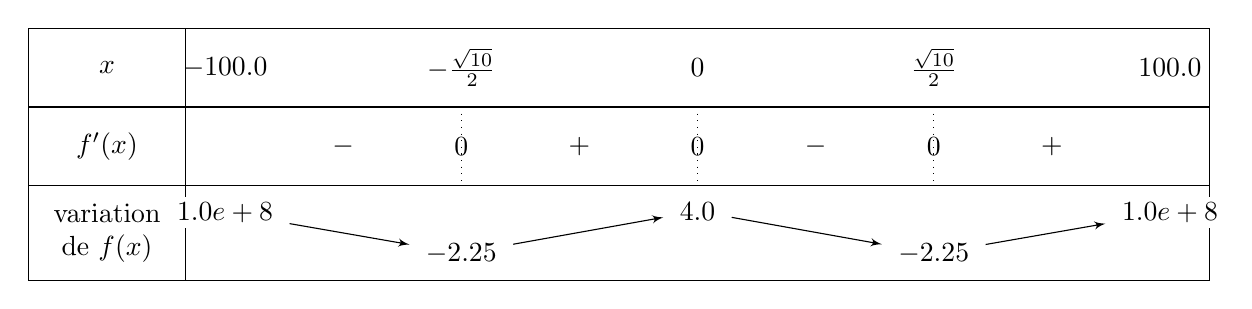
\begin{tikzpicture}
\tkzTabInit[espcl=3]{$x$ / 1 , $f'(x)$ / 1, variation de $f(x)$/1.2}
{$-100.0$,$- \frac{\sqrt{10}}{2}$,$0$,$\frac{\sqrt{10}}{2}$,$100.0$}
\tkzTabLine{,-,z,+,z,-,z,+}
\tkzTabVar{+/$1.0e+8$,-/$-2.25$,+/$4.0$,-/$-2.25$,+/$1.0e+8$}
\end{tikzpicture}
\end{document}